\documentclass{beamer}
\usepackage{config}

%Information to be included in the title page:
\title[Git collaboratif]{Git à plusieurs : mode d'emploi}
\author{Florian Legendre}
\institute{Université de Poitiers}
\date{Année 2020 - 2021}
\logo{
\includegraphics[scale=0.1]{images/UP.png}}


%%% ============================================================= %%%
%%% ====================== Début des diapos ===================== %%%
%%% ============================================================= %%%

\begin{document}

\frame{\titlepage}

\begin{frame}
\frametitle{Table of Contents}
\tableofcontents[hideallsubsections]
\end{frame}


%% --------------------- %%
%%        SECTION        %%
%% --------------------- %%
\AtBeginSection[]
{
  \begin{frame}
    \frametitle{Table of Contents}
    \tableofcontents[sectionstyle=show/hide,subsectionstyle=show/show/hide]
  \end{frame}
}
\section{Inviter des collaborateurs}

\begin{frame}
\frametitle{Gérer les droits de mise à jour}
Il y a trois scénarios possibles, qui dépendent de la configuration du ou des dépôts distants.
\medskip

\underline{Premier scénario:}\\
\smallskip
Vous êtes indiqué comme \textbf{collaborateur} sur la branche distante. En tant que collaborateur vous pouvez "pusher" les changements que vous voulez sans restriction ! Sauf si le projet fait partie d'une organisation...\\
\medskip
\textbf{ATTENTION pour les chefs de projet:} Cela nécessite d'avoir une très grande confiance en ses collaborateurs. En cas de doute une des solutions alors d'avoir une branche distante de développement
\end{frame}

\begin{frame}
\frametitle{Gérer les droits de mise à jour}

\begin{center}
\begin{figure}[h!]
    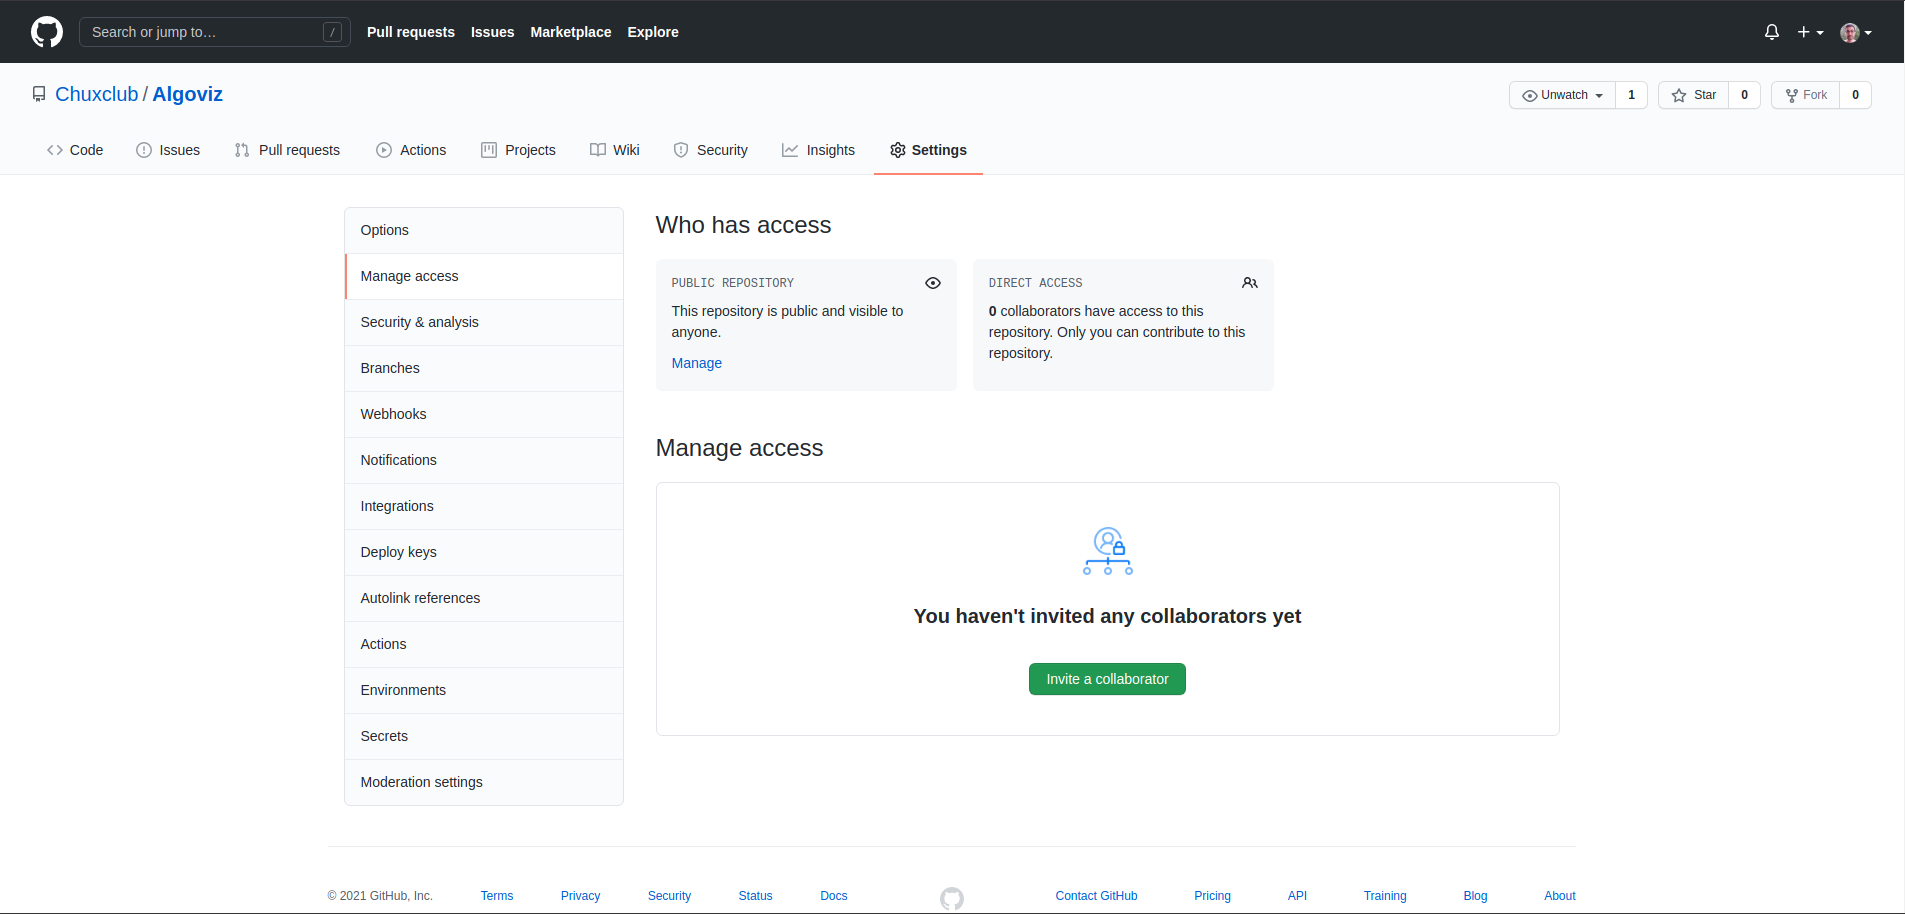
\includegraphics[scale=0.15]{images/droits_push/collaborator.png}
    \caption{Définir des collaborateurs sous GitHub}
\end{figure}
\end{center}

\end{frame}

\begin{frame}
\frametitle{Gérer les droits de mise à jour}

\underline{Second scénario:}\\
\smallskip

\begin{enumerate}
    \item Vous avez "\textbf{forké}" (càd copié) sous Github le projet d'une personne.
    \item Vous avez ensuite cloné ce fork.
    \item Vous avez travaillé sur ce clone et "pushé" vos projets sur votre fork distant.
    \item Vous pouvez ensuite faire un pull request directement sur l'interface GitHub.
\end{enumerate}

\normalsize
\end{frame}

\begin{frame}
\frametitle{Gérer les droits de mise à jour}
\begin{figure}[h!]
    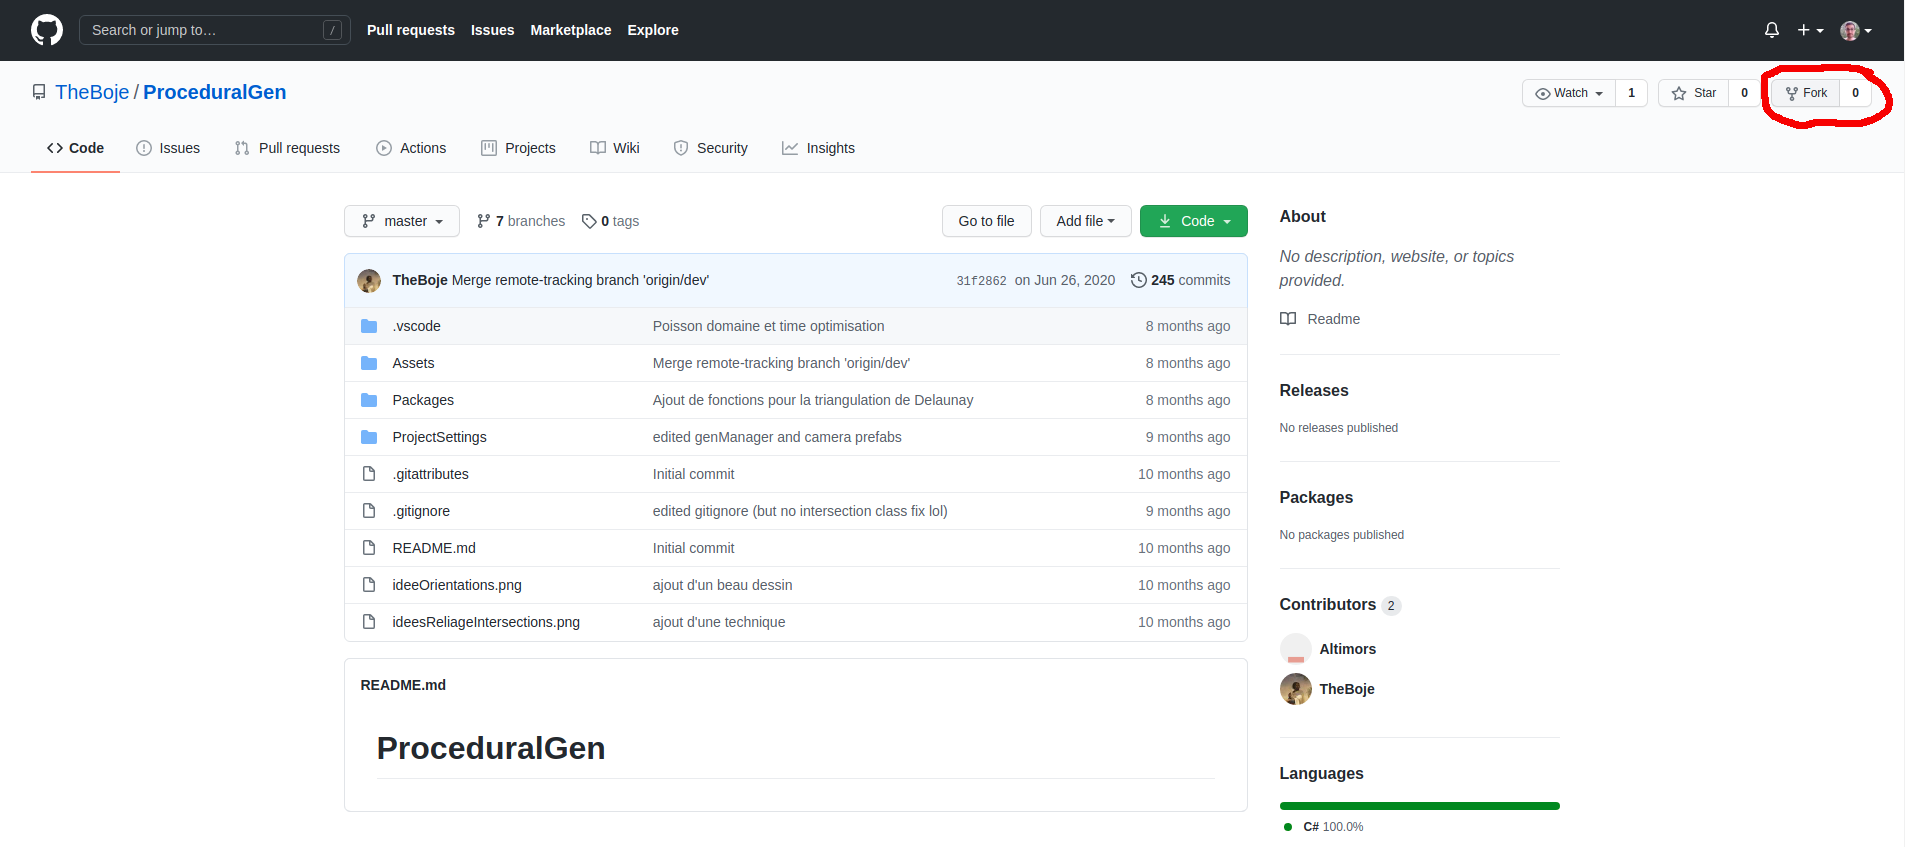
\includegraphics[scale=0.15]{images/droits_push/fork.png}
    \caption{Forker sous GitHub}
\end{figure}
\end{frame}

\begin{frame}
\frametitle{Gérer les droits de mise à jour}
\begin{figure}[h!]
    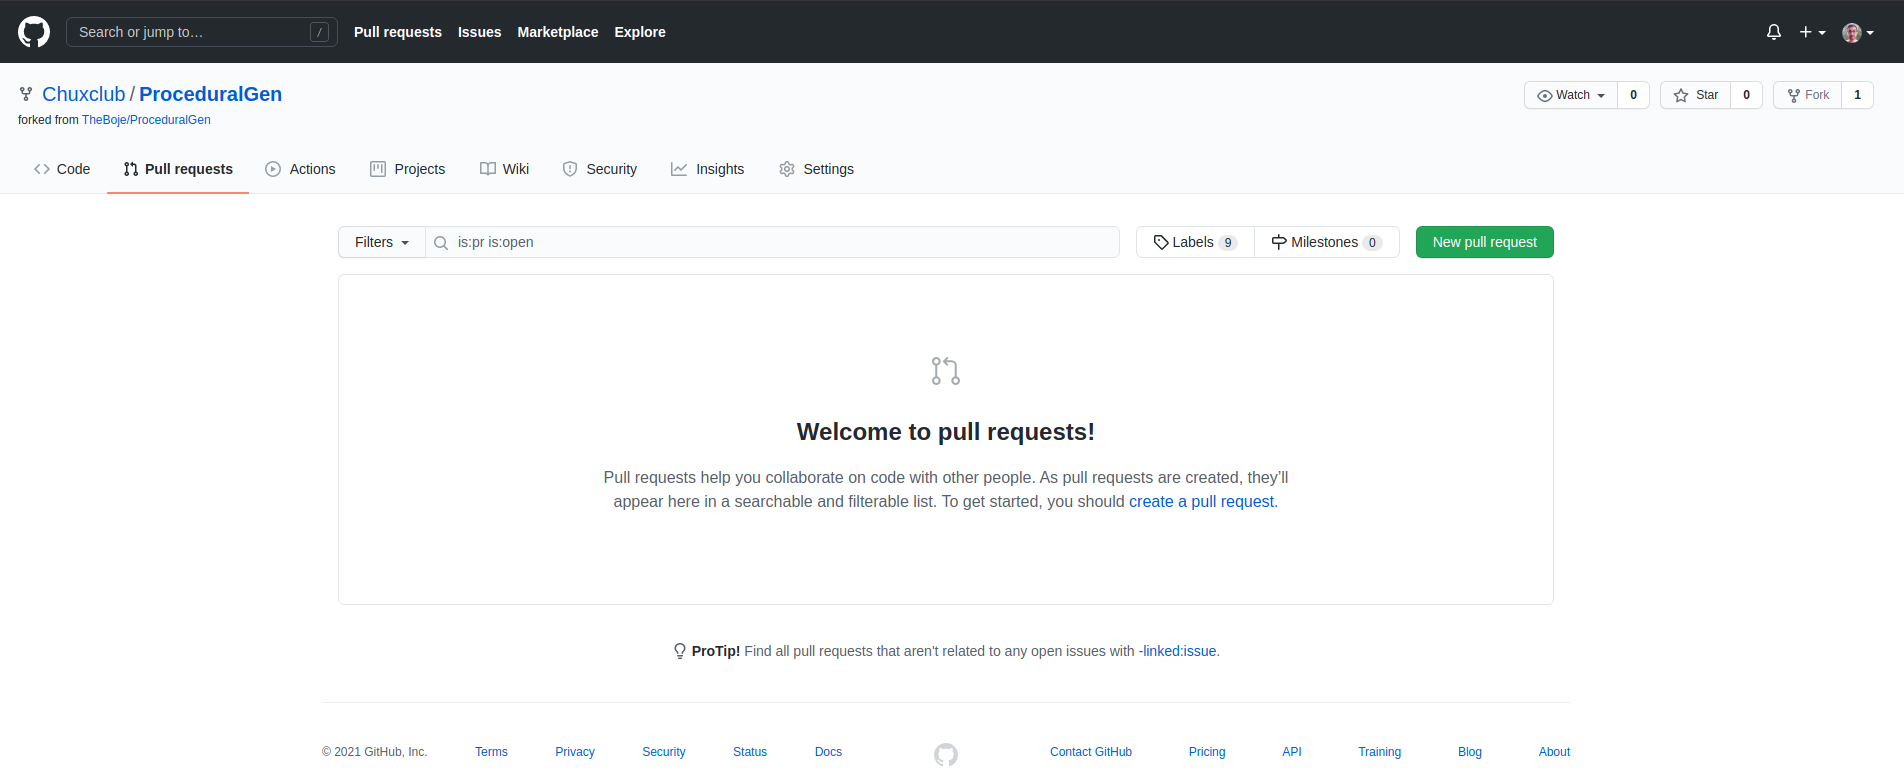
\includegraphics[scale=0.15]{images/droits_push/pull_request.png}
    \caption{Faire un pull request sous GitHub}
\end{figure}
\end{frame}


\begin{frame}
\frametitle{Gérer les droits de mise à jour}

\underline{Dernier scénario:}\\
\smallskip
Vous avez \textbf{cloné} le projet d'une personne. Vous avez ensuite travaillé dessus et vous vous rendez compte que vous souhaiteriez faire part de vos modifications à l'auteur...\\
\medskip

\begin{enumerate}
    \item Comme précédemment vous forkez
    \item Vous ajoutez une branche distante à votre clone: "git remote add <nom> <urlDeVotreDepot>" ou, plus brutal: "git remote rm origin" suivi de "git remote add origin <urlDeVotreDepot>"
    \item Vous pushez vos changements sur ce fork
    \item Vous faites un pull request comme précédemment
\end{enumerate}
\end{frame}


%% --------------------- %%
%%        SECTION        %%
%% --------------------- %%
\AtBeginSection[]
{
  \begin{frame}
    \frametitle{Table of Contents}
    \tableofcontents[sectionstyle=show/hide,subsectionstyle=show/show/hide]
  \end{frame}
}
\section{Gestion de conflits entre différentes versions}
\begin{frame}{Rappel de la notion de conflit de versions}
    
\end{frame}

\begin{frame}{Un conflit sur Git}
    
\end{frame}


\end{document}